\documentclass[12pt,letterpaper]{article}
\usepackage[utf8]{inputenc}
\usepackage[spanish]{babel}
\usepackage{graphicx}
\usepackage[left=2cm,right=2cm,top=2cm,bottom=2cm]{geometry}
\usepackage{graphicx} % figuras
% \usepackage{subfigure} % subfiguras
\usepackage{float} % para usar [H]
\usepackage{amsmath}
%\usepackage{txfonts}
\usepackage{stackrel} 
\usepackage{multirow}
\usepackage{enumerate} % enumerados
\renewcommand{\labelitemi}{$-$}
\renewcommand{\labelitemii}{$\cdot$}
% \author{}
% \title{Caratula}
\begin{document}

% Fancy Header and Footer
% \usepackage{fancyhdr}
% \pagestyle{fancy}
% \cfoot{}
% \rfoot{\thepage}
%

% \usepackage[hidelinks]{hyperref} % CREA HYPERVINCULOS EN INDICE

% \author{}
\title{Caratula}

\begin{titlepage}
\begin{center}
\large{UNIVERSIDAD PRIVADA DE TACNA}\\
\vspace*{-0.025in}
\begin{figure}[htb]
\begin{center}

\includegraphics[width=8cm]{./Imagenes/logo}
\end{center}
\end{figure}
\vspace*{0.15in}
INGENIERIA DE SISTEMAS  \\

\vspace*{0.5in}
\begin{large}
TITULO:\\
\end{large}

\vspace*{0.1in}
\begin{Large}
\textbf{INFORME DE LABORATORIO No 01} \\
\end{Large}

\vspace*{0.3in}
\begin{Large}
\textbf{CURSO:} \\
\end{Large}

\vspace*{0.1in}
\begin{large}
INTELIGENCIA DE NEGOCIOS \\
\end{large}

\vspace*{0.3in}
\begin{Large}
\textbf{DOCENTE(ING):} \\
\end{Large}

\vspace*{0.1in}
\begin{large}
 Patrick Cuadros Quiroga\\
\end{large}

\vspace*{0.2in}
\vspace*{0.1in}
\begin{large}
Alumna: \\
\begin{flushleft}
Flor de María Condori Gutierrez		\hfill	(2015053227) \\

\end{flushleft}
\end{large}
\end{center}

\end{titlepage}


\tableofcontents % INDICE
\thispagestyle{empty} % INDICE SIN NUMERO
\newpage
\setcounter{page}{1} % REINICIAR CONTADOR DE PAGINAS DESPUES DEL INDICE

\section{Actividad No 01 – Conectar a SQL Server desde Power BI Desktop} 



\begin{enumerate}[1.]
	\item  En el cuadro de dialogo base de datos SQL Server, en la casilla servidor tipear (local), en la casilla Base de datos (opcional) / Database (optional), tipear AdventureWorks2017, y hacer clic en OK.
	

	\begin{center}
	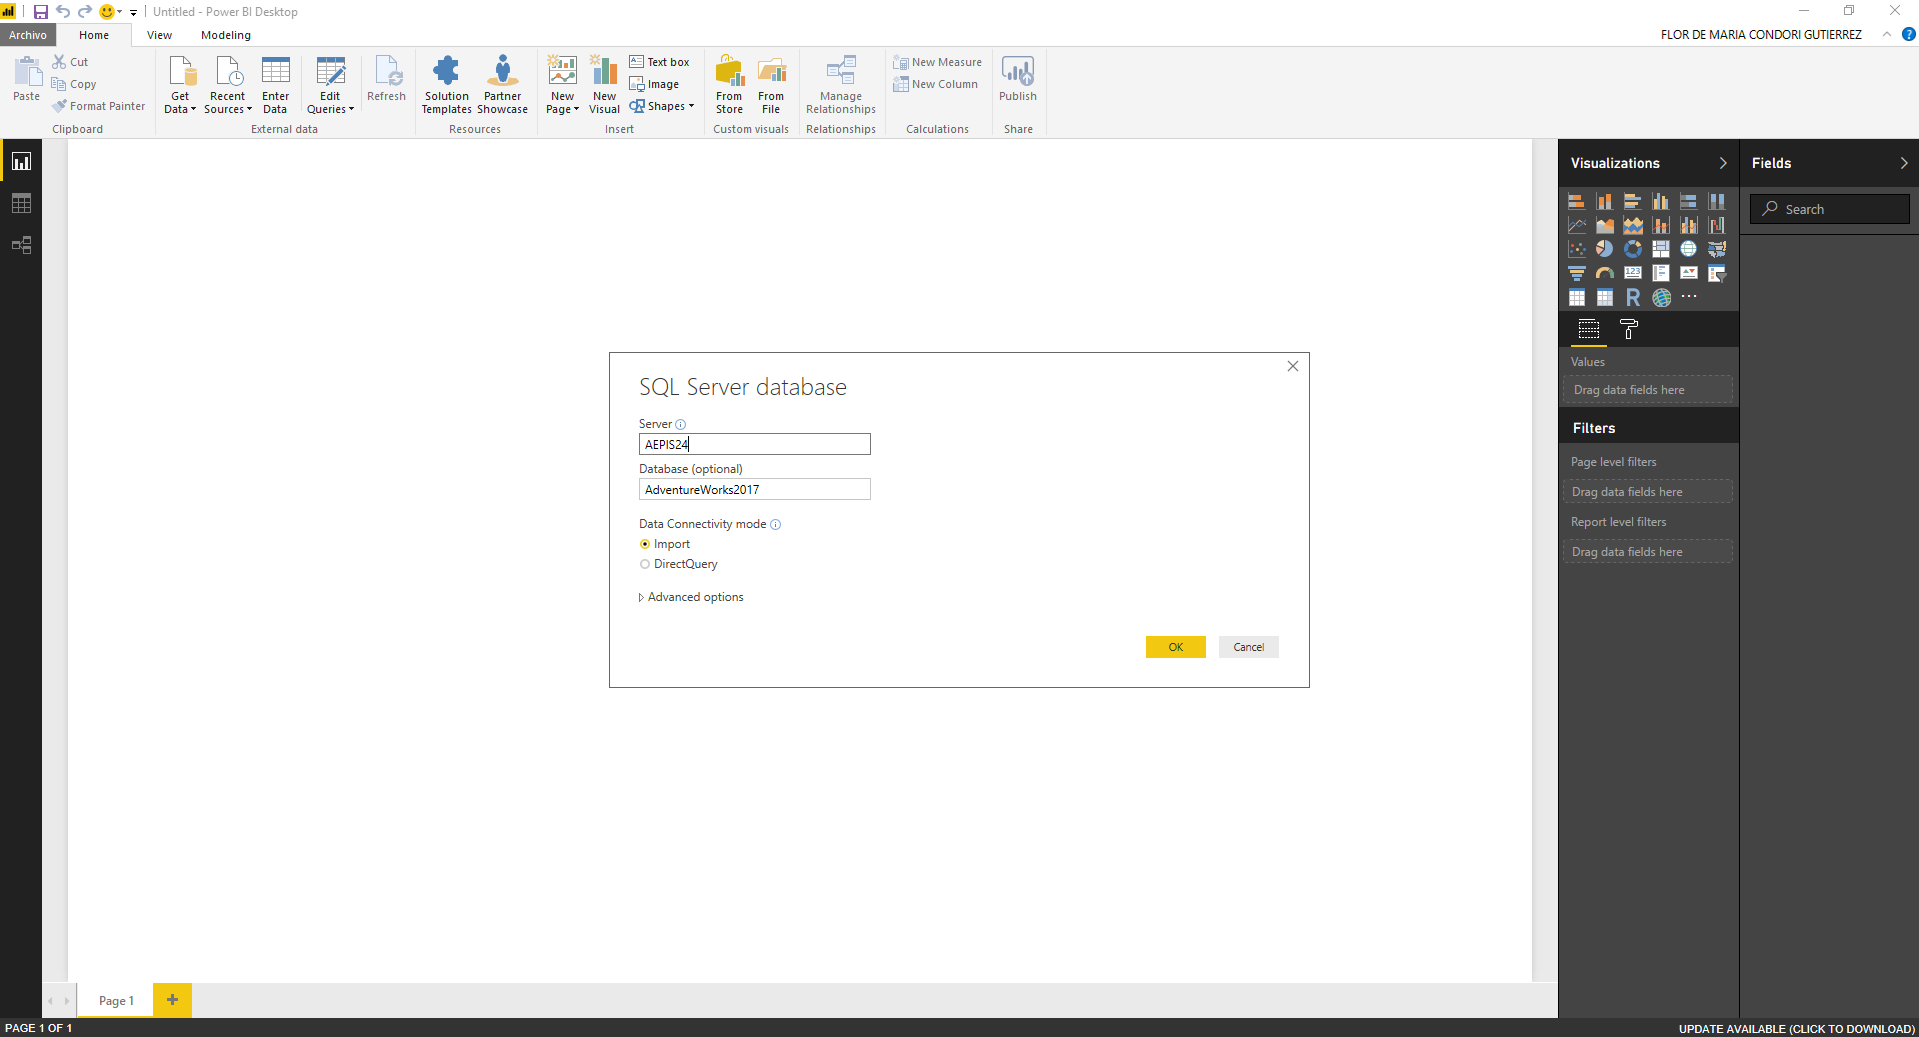
\includegraphics[width=16cm]{./Imagenes/11} 
	\end{center}


	\item  En el cuadro de dialogo Navegador (Navigator), seleccionar el check en Sales.vSalesPerson, y entonces hacer click en Cargar (Load).

	\begin{center}
	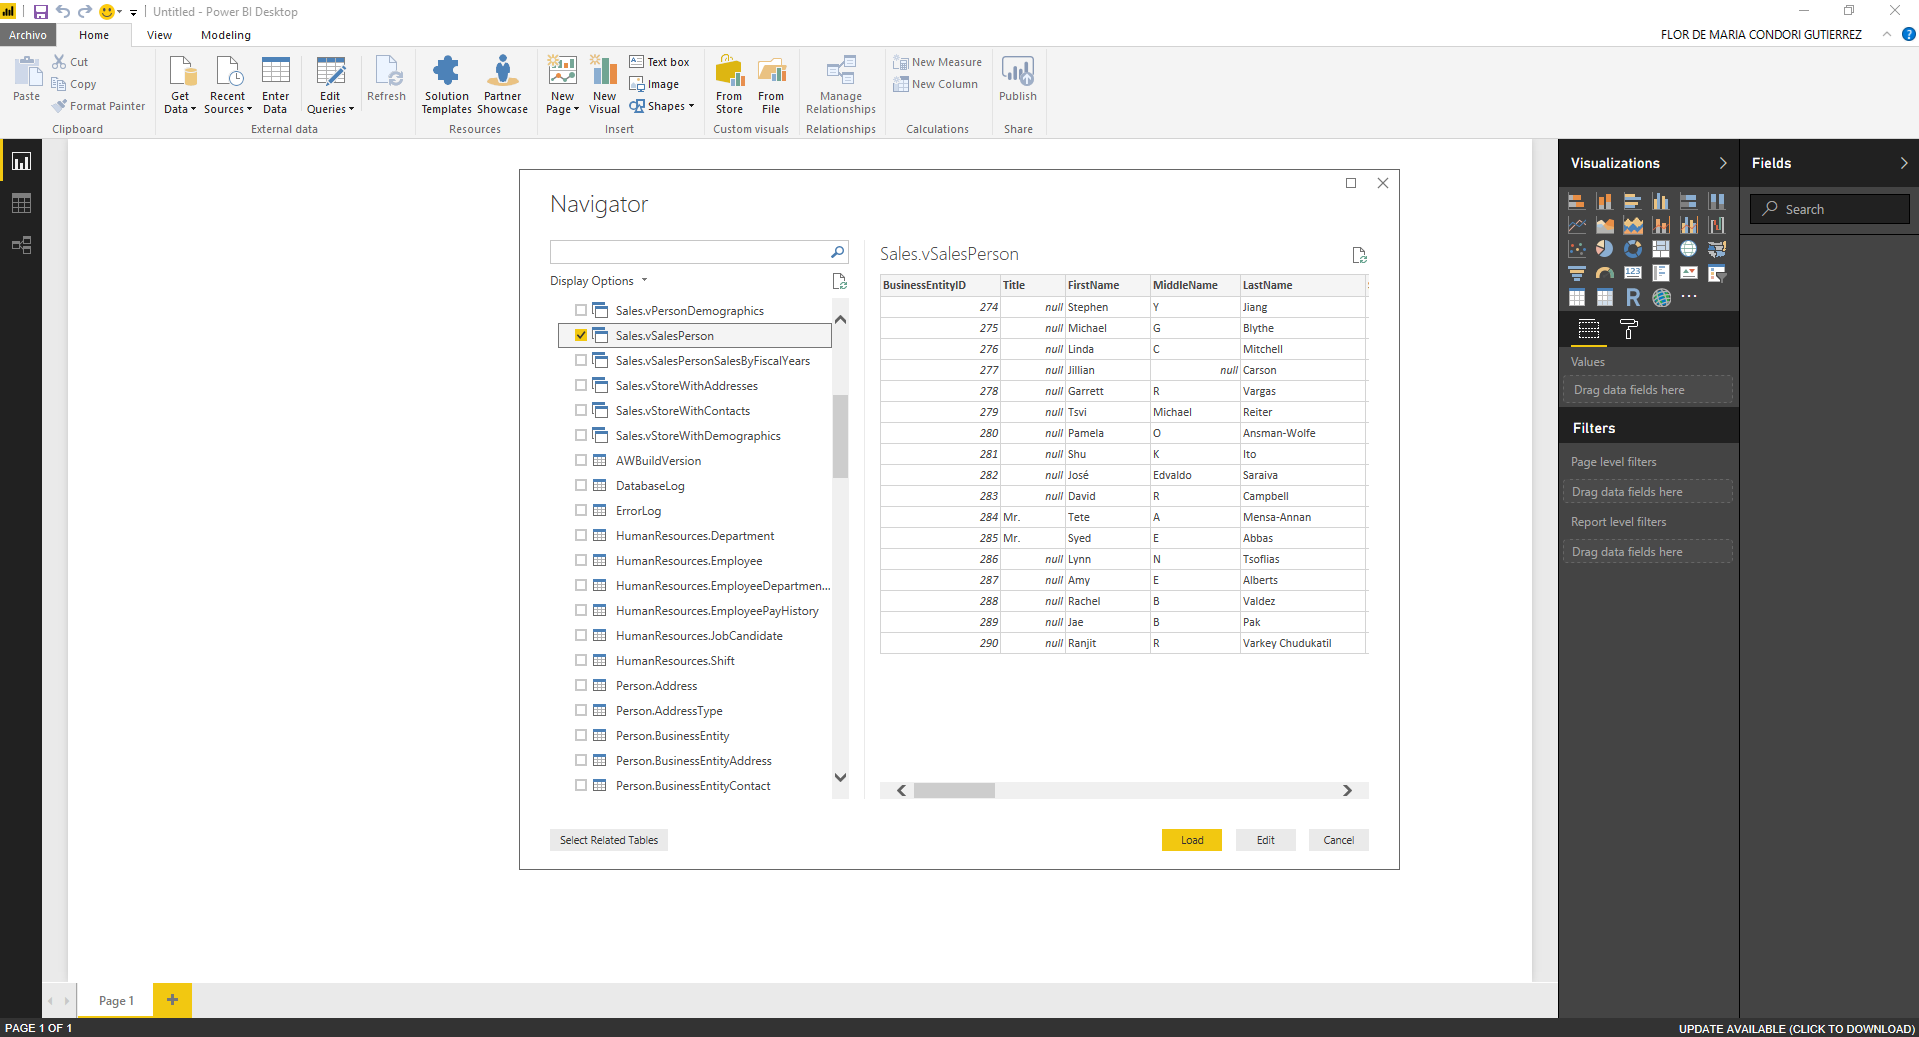
\includegraphics[width=16cm]{./Imagenes/12} 
	\end{center}


	\item Expandir opciones Avanzadas, en la casilla sentencia SQL (opcional, base de datos requerida), tipear la siguiente consulta, y luego hacer click en OK:
	\\
	\\SELECT TOP 10 P.ProductID, P.Name AS Product, SUM(CAST(LineTotal AS decimal(18,2))) AS LineTotal FROM 	Purchasing.PurchaseOrderDetail AS POD INNER JOIN Production.Product AS P ON POD.ProductID = P.ProductID GROUP BY P.ProductID, P.Name ORDER BY LineTotal DESC

	\begin{center}
	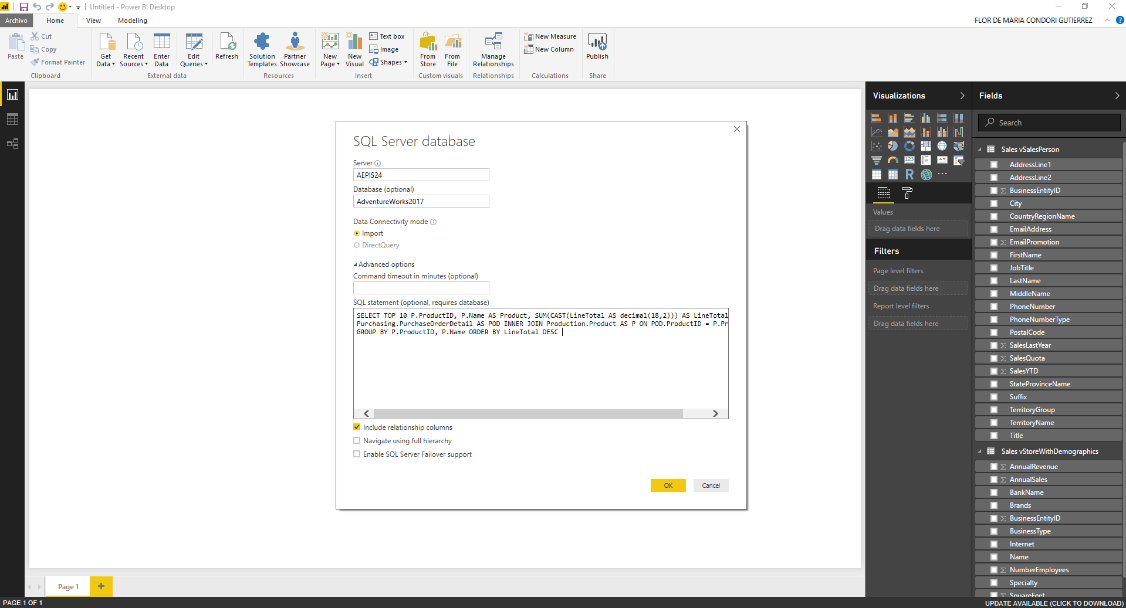
\includegraphics[width=16cm]{./Imagenes/13} 
	\end{center}

\end{enumerate}





\section{Actividad No 02 – Adicionar Gráficos al Reporte} 

\begin{enumerate}[1.]
	\item Arrastrar el campo SalesYTD a la casilla Valores (Values). El gráfico se llenará con datos.
	\\
	\\

	\begin{center}
	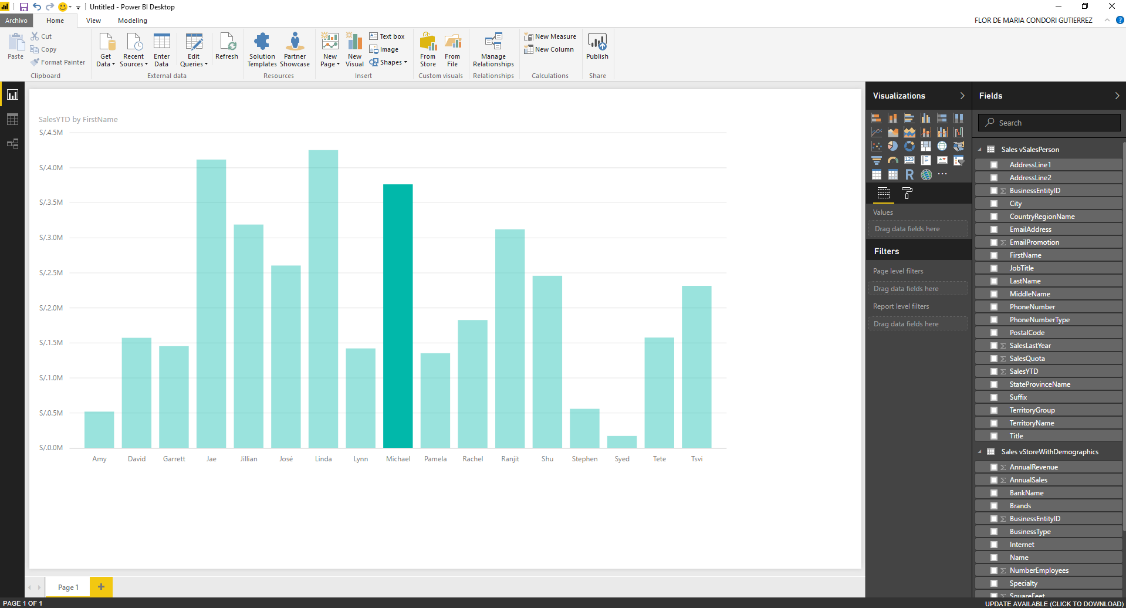
\includegraphics[width=16cm]{./Imagenes/21} 
	\end{center}

	\item Cambiar el color para Jae, Linda, y Michael a rojo.
	\\
	\\

	\begin{center}
	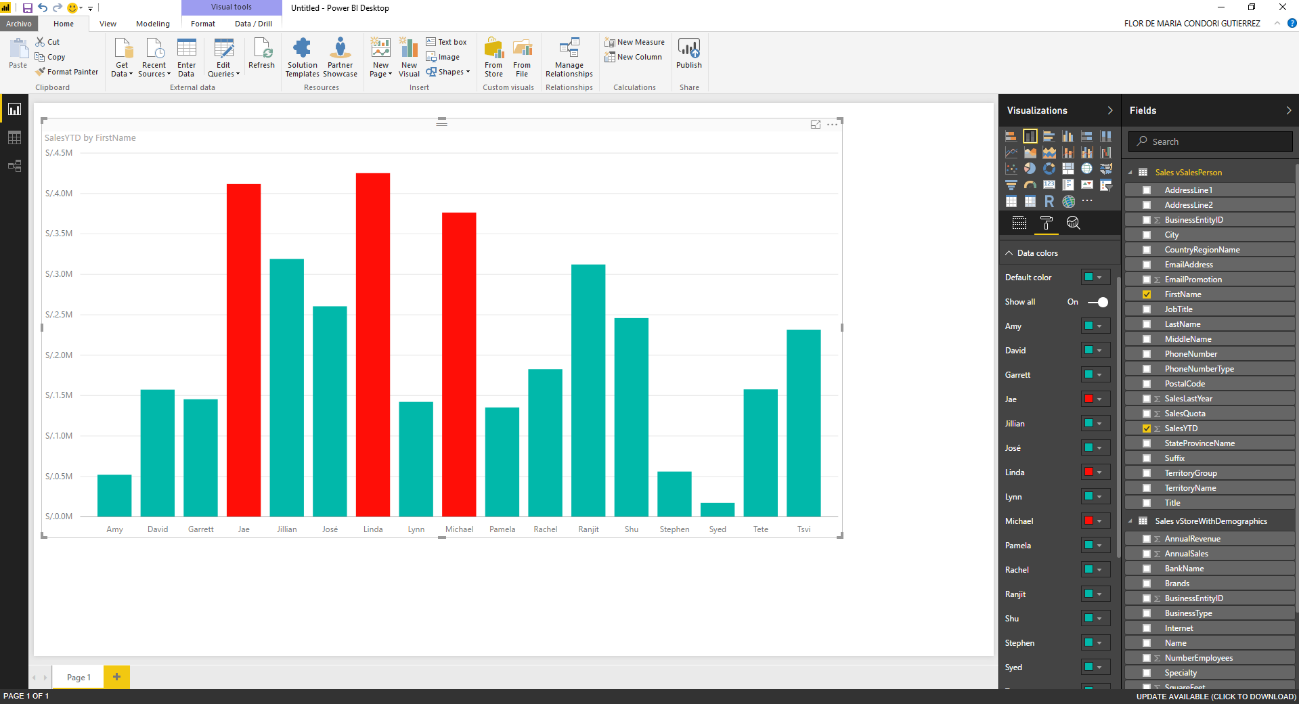
\includegraphics[width=16cm]{./Imagenes/22} 
	\end{center}

	\item En el panel Campos, hacer click en la elipsis (…) contigua a AnnualRevenue, y hacer click en Renombrar (Rename). Tipear Beneficios anuales luego presionar Enter.
	\\
\\
	
	\begin{center}
	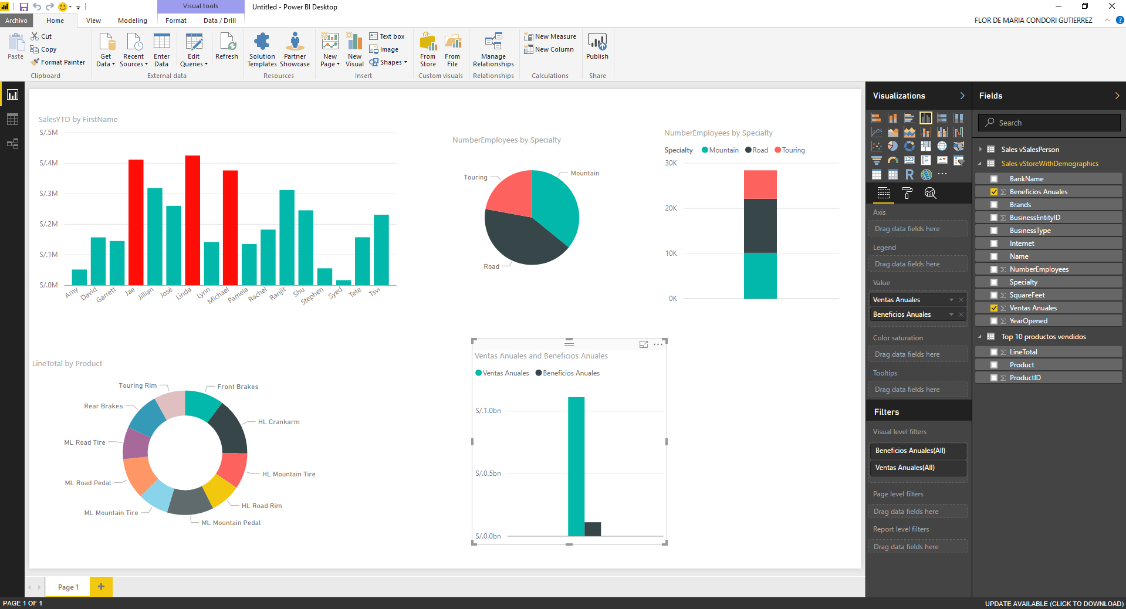
\includegraphics[width=16cm]{./Imagenes/23} 
	\end{center}


	\item Expandir la Información de página (Page Information), y en la casilla Nombre tipear Ventas. Hacer click en el área de reporte y apreciar que el nombre ha cambiado en la pestaña al final del reporte.
	\\
	\\
	\begin{center}
	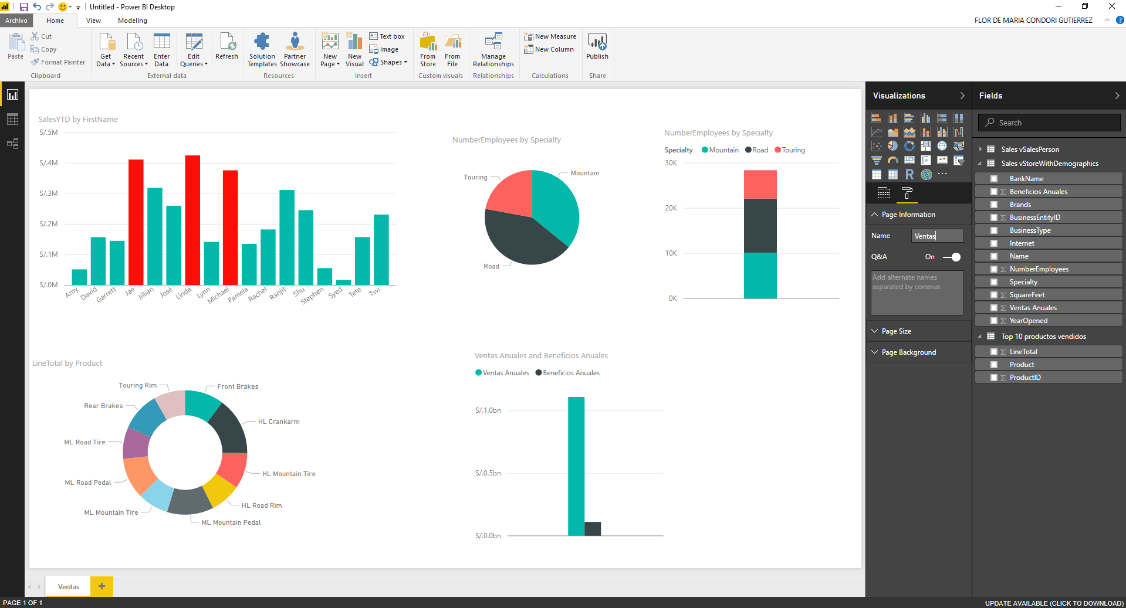
\includegraphics[width=16cm]{./Imagenes/24} 
	\end{center}

	\item En el menu Archivo (File menu), hacer click en Guardar (Save), crear un directorio Power BI, y guardar el archive como Ventas de Adventure Works Sales.
	\\
	\\
	\begin{center}
	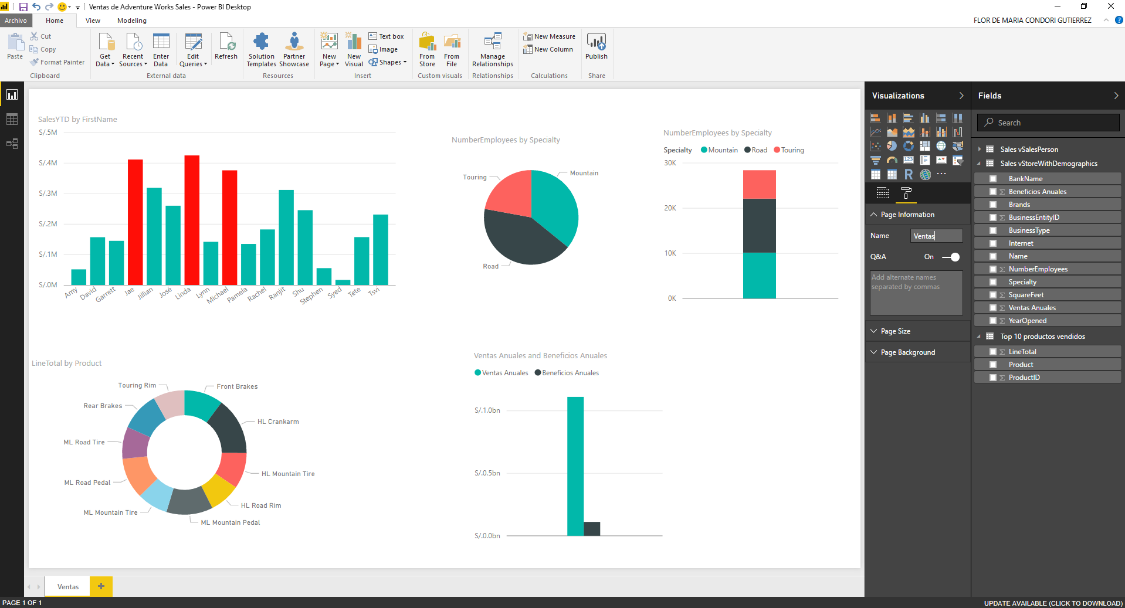
\includegraphics[width=16cm]{./Imagenes/25} 
	\end{center}

\end{enumerate}






\end{document}
